\documentclass{article}

\usepackage[
  paperheight=8.5in,
  paperwidth=5.5in,
  left=10mm,
  right=10mm,
  top=20mm,
  bottom=20mm]{geometry}
\usepackage[utf8]{inputenc}

\usepackage{graphicx}
\usepackage{wrapfig}
\usepackage[bottom]{footmisc}
\usepackage{listings}
\usepackage{enumitem}

\usepackage{wrapfig}
\usepackage{ragged2e}

\usepackage{array}
\usepackage[table]{xcolor}
\usepackage{multirow}
\usepackage{booktabs}
\usepackage{hhline}
\definecolor{palegreen}{rgb}{0.6,0.98,0.6}

\usepackage{amsmath}
\usepackage{amssymb}
\usepackage{multicol}
\usepackage{lipsum}
\usepackage{hyphenat}
\PassOptionsToPackage{hyphens}{url}
\usepackage{url}

\usepackage{rotating}

%\usepackage{xeCJK}

%% support use of straight quotes in code listings
\usepackage[T1]{fontenc}
\usepackage{textcomp}
\usepackage{listings}
\lstset{upquote=true}

%% for shrinking space between lines
\usepackage{setspace}

\newcommand*{\affaddr}[1]{#1} % No op here. Customize it for different styles.
\newcommand*{\affmark}[1][*]{\textsuperscript{#1}}
\newcommand*{\email}[1]{\small{\texttt{#1}}}
\newcommand{\tarot}{\textsc{Tarot}}
\renewcommand*\contentsname{\centering Table of Contents}

\renewcommand{\footnoterule}{%
  \kern -3pt
  \hrule width \textwidth height 0.5pt
  \kern 2pt
}

% remove date
\date{}

\usepackage{titlesec}
\titleformat*{\section}{\large\bfseries}
\titleformat*{\subsection}{\normalsize\bfseries}
\titleformat*{\subsubsection}{\normalsize\bfseries}

\usepackage{biblatex}


\usepackage{algorithm}
\usepackage{algpseudocode}

\addbibresource{references.bib}

\title{Enhancing Learning in CS Capstone Courses Through Advanced Project Matching\footnote{\protectCopyright \copyright 2024 by the Consortium for Computing Sciences in Colleges.
Permission to copy without fee all or part of this material is granted provided
that the copies are not made or distributed for direct commercial advantage,
the CCSC copyright notice and the title of the publication and its date appear,
and notice is given that copying is by permission of the Consortium for
Computing Sciences in Colleges.  To copy otherwise, or to republish, requires
a fee and/or specific permission.
}
}

\author{
Barbara Martinez Neda, Jason Lee Weber,\\ Sergio Gago-Masague, and Jennifer Wong-Ma\\
Department of Computer Science\\
University of California, Irvine\\
Irvine, CA 92617\\
\email{\{barbarm,weberjl,sgagomas,jwongma\}@uci.edu}}


\begin{document}
\maketitle
\thispagestyle{empty}
\pagestyle{empty}

\begin{abstract}

% background
Optimal group formation and project matching are critical and challenging tasks for instructors.
% methods
We developed the Student-Project Matching Tool to optimize these processes and piloted it in a Computer Science Capstone course at the University of California, Irvine. The tool ensures that the team formation process balances individual preferences, project compatibility, and the overall performance potential of each team by considering students' skills and interests and sponsor projects' needs to maximize teams' success.
% results
Student perspectives and feedback showed an increase in student satisfaction with their team and the project they were matched to. Similarly, positive sponsor evaluations of the teams demonstrated that sponsors were pleased with the teams they were matched to.
% conclusion
This tool provides the basis for effective team formation and project matching in Capstone courses, with a focus on maximizing student learning outcomes, real-world experiences, student-project ownership, and the number of fulfilled skills that each project requires for completion.


\end{abstract}

\section{Introduction}


For many decades, researchers and instructors have aimed to optimize team formation in student engineering projects. Brickell et al found that allowing for the self-formation of teams led to negative student attitudes towards their courses, instructors, projects, and more~\cite{brickell_assigning_1994}. With justification for instructor-created teams established, the focus has shifted towards optimizing the team formation process. To this end, Layton et al wrote a digital tool in an attempt to computationally pick the ``best'' teams by asking students questions and weighting their responses \cite{layton_design_2010}. However, these approaches' matching strategies are solely dependent on the variables each instructor or researcher chooses to incorporate in their algorithm, not taking into account project needs directly. For instance, Smyser and Jaeger found that a key factor of success in capstone teams is in students' passion and ownership of their project~\cite{smyser_how_2015}. 
Therefore, it is crucial that we not only optimize the matching of students into teams, but also the matching of students to projects, ensuring that all project skills requirements can be fulfilled.

Since Conn and Sharpe in 1993~\cite{conn_industry-sponsored_1993}, it has become commonplace for many capstone courses to match student teams to industry-sponsored projects. However, this introduces another layer of complexity to the team-formation and matching process, as industry stakeholders have their own set of team requirements. Thus, any computational team-forming tool must not only optimize student-centered variables but also stakeholder-centered variables.

\subsection{Goals}

The primary goal of this study was to design and test the Student-Project Matching Tool (SPMT) for a CS Software Engineering (SWE) Capstone course. This innovative platform is designed to aid instructors in forming student teams and matching them with industry-sponsored projects to improve student outcomes. Specifically, we designed the SPMT to support the following outcomes: (i) increased student-project buy-in/ownership, (ii) broadened student skillsets, and (iii) fulfilled project skills requirements.


We tested our desired outcomes by piloting the SPMT in a six-month-long CS SWE Capstone course at the University of California, Irvine (UCI) during the 2022-2023 academic year to form student groups and assign them to the best industry-sponsored project match. The SPMT determined the best match by considering students' interests and skills in SWE topics relevant to each project, and conversely ensuring that the skills across all students in a group collectively met the needs of the project they were matched to.




\section{Student-Project Matching Tool}

The SPMT consists of three parts: data collection, the Student Project Matching (SPM) Recommender, and the final set of teams (see Figure \ref{fig:SPM}). Prior to data collection, we needed to first define what skills are currently valued by SWE employers. To do this, we identified six main categories of SWE jobs and searched for them on three popular job-search websites \cite{noauthor_job_nodate-1, noauthor_job_nodate, noauthor_jobs_nodate}. We then selected the first ten job postings for each category on each website and extracted the SWE skills mentioned in their descriptions. Skills that were included in 70\% of a category's job postings were then selected for incorporation into the data collection step of the SPMT. Lastly, the industry partners reviewed the full list of SWE categories and the resulting skills, which are listed in Table \ref{tab:student_skills_survey}.

\begin{table}[t]
    \centering
    \scriptsize
    \begin{tabular}{p{1.5cm}p{1.5cm}p{1.5cm}p{1.5cm}p{1.5cm}p{1.8cm}}
    \hline
        \textbf{Front-end - Web} & \textbf{Front-end - Mobile} & \textbf{Back-end} & \textbf{Databases} & \textbf{ML/AI} & \textbf{Data Science} \\ \hline
        UI/UX & UI/UX & Java & Oracle & Python & Python \\ 
        HTML & Kotlin & PHP & MySQL & OO Lang. & JavaScript \\ 
        CSS & Java & Python & PostreSQL & PyTorch & R \\ 
        Javascript & Swift & C\# & MongoDB & TensorFlow & Tableau \\ 
        React & Unix OS & Ruby & ~ & AWS & Power BI \\ 
        Angular & ~ & REST APIs & ~ & Docker & Spark \\ 
        Vue.js & ~ & TCP/IP & ~ & ~ & Hadoop \\ \hline
    \end{tabular}
    \caption{Skills, tools and frameworks in each SWE category for which students had to rank their level of familiarity in the Student Intake Survey.}
    \label{tab:student_skills_survey}
\end{table}




\subsection{Data Collection}
Data collection was comprised of two student surveys and one project sponsor survey. In the Student Intake Survey, students were asked to indicate their level of confidence in each of the SWE skills listed in Table \ref{tab:student_skills_survey}, as well as which skills they wished to develop or continue improving. In the Sponsor Intake Survey, industry sponsors determined what languages, frameworks, and technologies would be needed for each project. Industry sponsors also submitted 3-minute video project descriptions, and students were asked to rank their interest in each project on the Student Project Ranking Survey. 


\subsubsection{Sponsor Intake Survey}
The Sponsor Intake Survey consisted of 38 questions to learn about the sponsor and their project. Five questions collected sponsor and project information and the mentors' availability to provide technical guidance. The remaining 33 questions asked for the level of relevance of various programming languages, frameworks, and technologies which mapped to the SWE categories in Table \ref{tab:student_skills_survey}.


\subsubsection{Student Intake Survey}

The Student Intake Survey consisted of 72 questions, and its main goal was to understand students' backgrounds and technical goals. Five questions captured students' personal information and demographics. Eight questions captured students' background and goals, focusing on confidence in the field, SWE topic interest, courses taken and grades obtained, and interest in being a team lead. The remaining 59 questions focused on capturing a students' technical background and soft skills. Specifically, the questions focused on students' experience level across a variety of programming languages, frameworks, and technologies. Questions were formatted as single-response multiple-choice, multiple-response multiple-choice, and Likert scales.



\subsubsection{Student Project Ranking Survey}
Industry sponsors were asked to create short video and text summaries of their projects to pitch to students. Students were then asked to fill out the Student Project Ranking Survey, which consisted of 14 questions and the sponsors' video and text descriptions. Students ranked their level of interest for each of the sponsor projects on a 3-point Likert scale (High Interest, Somewhat Interested, No Interest). In the remaining questions, they were able to propose their own project, list potential team members, and express interest in being a team lead.

\begin{figure}
    \centering
    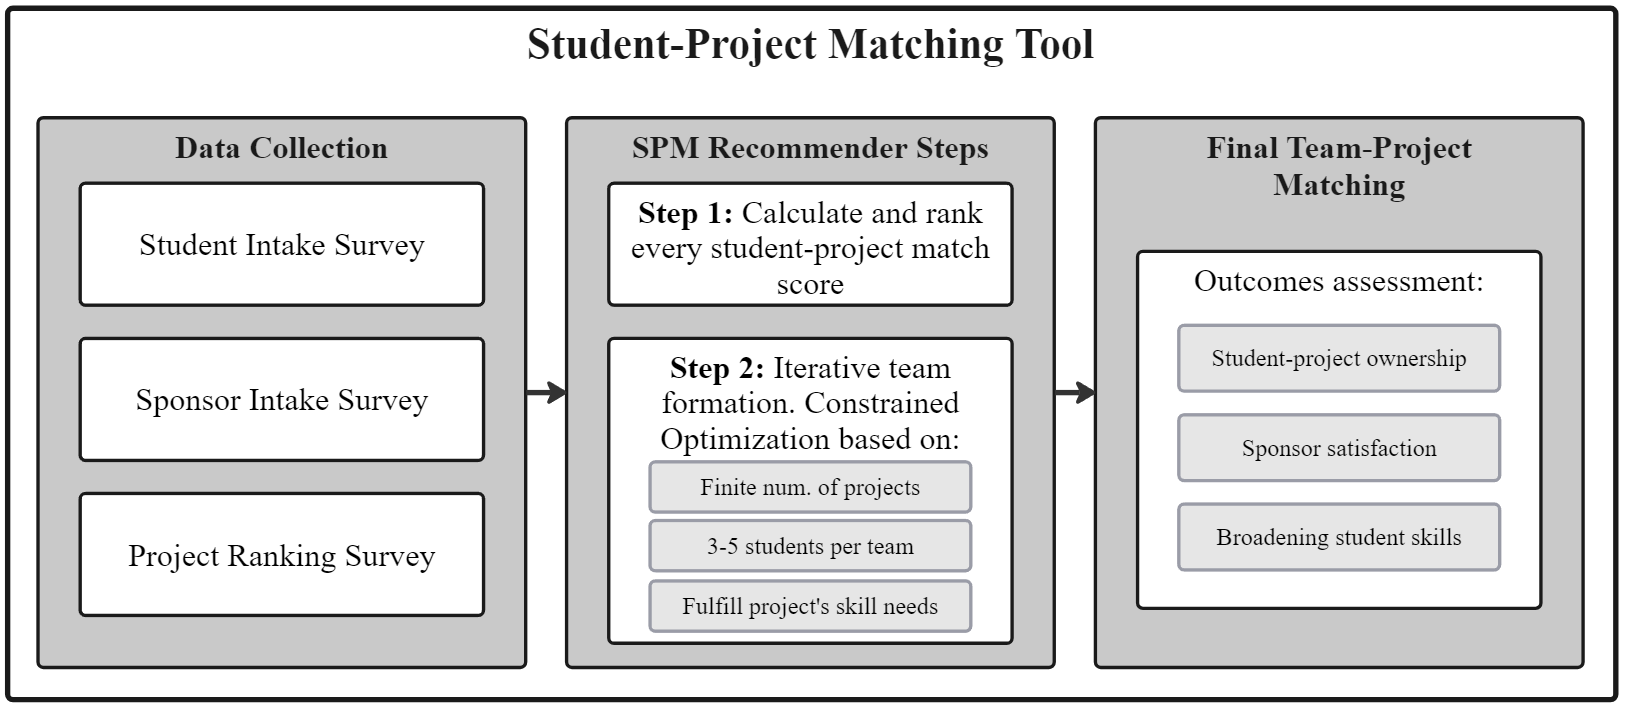
\includegraphics[width=1\linewidth]{Pictures/SPM_Figure.png}
    \caption{Overview of tasks performed by the Student-Project Matching Tool. }
    \label{fig:SPM}
\end{figure}

\subsection{The SPM Recommender}
The SPM Recommender was designed to measure students' fitness and rank them accordingly for each available Sponsor Project by assessing their skills, interests, and knowledge identified through the Intake Surveys. The SPM Recommender was comprised of two steps implemented using Python.

During Step 1, the SPM Recommender imported the responses to the three surveys, iterated through every available industry-sponsored project, and calculated a project score for each student. This score was based on the student's interest and skill levels for each SWE category, and the SWE category's level of relevance for each project. 

In Step 2, student groups were formed and matched while meeting the following constraints (also outlined in Figure \ref{fig:SPM}): Each group must have a maximum of 5 students, only one group can be assigned to each project, there is a finite number of projects (ten for the piloted capstone course), and the project's skill needs must be fulfilled.
These constraints collectively guided the team formation process, striking a balance between individual preferences, project compatibility, and the overall performance potential of each team.



\section{Results and Discussion}


In 2023, we conducted a six-month CS Capstone course at UCI where we piloted the use of the SPMT. We then evaluated the effectiveness of the SPMT by gathering feedback from both students and sponsors. We compared this feedback to that gathered in the 2022 course taught by the same instructor when students were placed in teams based solely on their project and team member preferences. Results show that the SPMT maximized the opportunity for students to learn new skills since it considered student interests in the matching process, and it increased student satisfaction with their groups and projects. The SPMT not only helped to match students with better educational projects but also acted as a catalyst in boosting student-project ownership and a deeper understanding of the SWE profession. This also led to higher sponsor satisfaction with the group formation and project matching during the piloting period.




\subsection{Sponsor Feedback}
Sponsor feedback during the pilot was compared to feedback during the previous year before the SPMT was introduced. At the end of the first term in both offerings, sponsors had the opportunity to review their team's performance.

In the year before the SPMT, two out of the six project reviews expressed discontent with student progress and preparedness. Industry sponsors stated that ``the students' readiness to do hands-on programming was less than expected'' and ``they veered off of the original requirements which led to a gap between what they developed and what was expected''. Additionally, only one sponsor expressed satisfaction working with their team.


The benefits of the switch to SPMT in 2023 were evident in the shift of general sentiment to much more positive reviews during the feedback stage. Out of nine submitted team reviews, four sponsors recognized their team's efforts by sharing that the teams are ``really scrappy'', ``doing a great job'', ``show high levels of enthusiasm'', and ``quick learners''. In contrast, only one comment pointed to areas of improvement, saying that ``communication could be better'', which was not one of the skills targeted by SPMT.
The shift to primarily positive feedback from sponsors shows the teams' ability to meet their sponsor's expectations, highlighting the value of the team matching tool.


\subsection{Qualitative Student Feedback}
Student course evaluations provided a means of understanding student experiences before and after the introduction of the Student-Project Matching Tool. 

In 2022, 15 out of 29 students filled out the survey. One question asked students to mention any aspects of the course that could be modified to improve their learning. Of the 15 responses, three mentioned that team and project matching could be improved. 

Overall, feedback pointed to the common weaknesses encountered when only considering project and team member preferences in the matching process.

In 2023, 43 out of 47 students filled out the survey. The total number of responses almost tripled due to the larger class size and higher response rate. Despite a higher number of participants, only two responses to the improvements question mentioned the lack of technical knowledge for the project. This type of comment was expected because the tool was designed to challenge students to acquire new skills that they showed interest in.







\section{Conclusion and Future Work}


In conclusion, the SPMT pilot in a Computer Science Capstone course has demonstrated positive outcomes, enhancing student satisfaction with skillset growth, team formation, and project assignments. Acknowledging the initial limitations in the availability of industry-sponsored projects during the pilot, our future work focuses on diversifying opportunities and expanding the pool of available projects. We plan to optimize the SPMT by testing various matching algorithms to maximize student learning when limited projects are available. Additionally, new, more targeted feedback surveys will be designed to gather deeper insights for ongoing refinement of the SPMT. 
The SPMT shows promise as a tool for enhancing team formation and project matching in SWE, and ongoing efforts should continue to focus on improving student learning outcomes and real-world experiences.


\medskip

\printbibliography

\end{document}
